\documentclass[../main.tex]{subfiles}

\begin{document}
\section{UCB-BAR: Rocket Chip Generator}
\begin{figure}
    \centering
    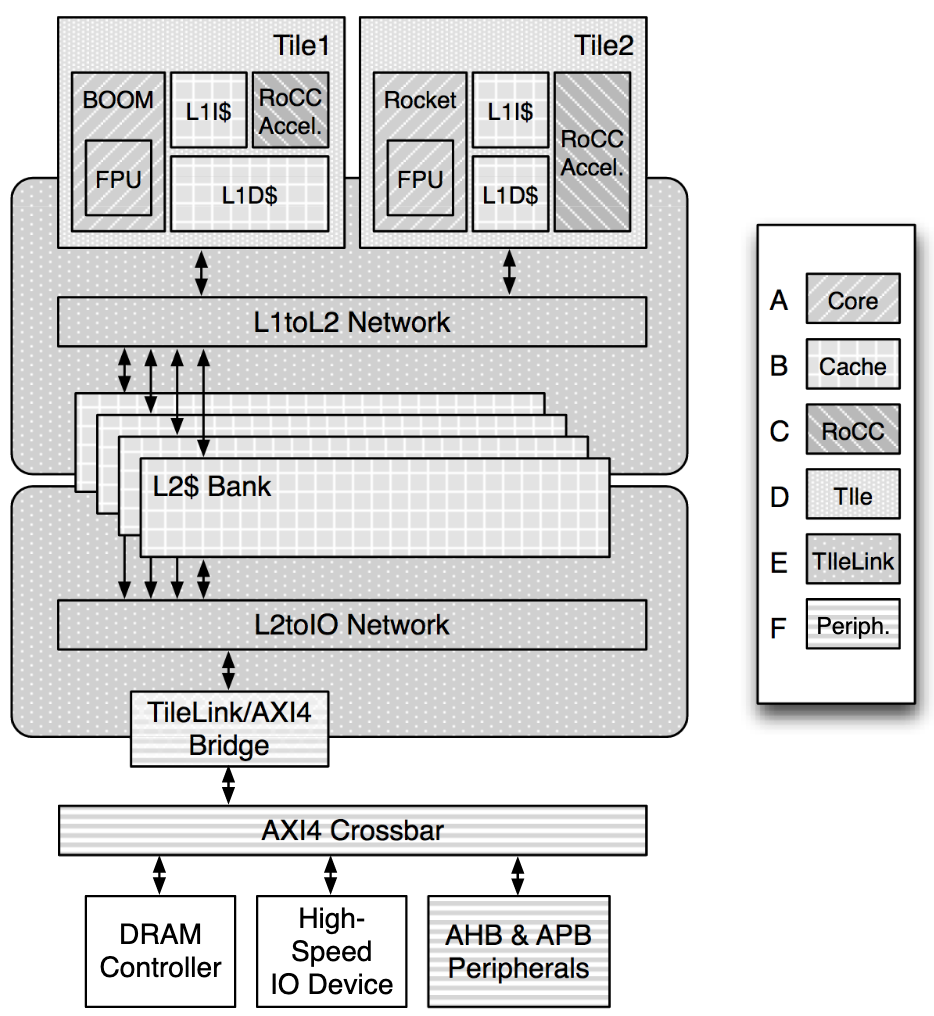
\includegraphics[scale=.5]{pngs/RocketChipGeneratorLayout.png}
    \caption{Rocket Chkp Pipeline\cite{Asanović:EECS-2016-17}}
    \label{fig:RocketCipGen}
\end{figure}
The Rocket Chip Generator was developed at the University of California, Berkeley (UCB). The generator is maintained by the Chips Alliance group. The generator produces a system on chip (SOC) with caches and processor tiles. See Figure \ref{fig:RocketCipGen} for a high level view SOC generated by the Rocket Chip Generator. % FIXME look for refs on the Chip Alliance   

%The Rocket Core was generated by using the Rocket Chip Generator. The Rocket Chip Generator was developed by UC. Berkeley and is maintained by the CHIPS Alliance. Figure \ref{fig:RocketCipGen} shoe a high level overview of a default Rocket Chip. 

\subsection{Generic Rocket Chip}
The following is an overview of the SOC generated by the Rocket Chip Generator. At the lowest level is the tiles, top of figure \ref{fig:RocketCipGen}. A Tile will contain a RISC-V processor L1 data cache, L1 instruction cache. A Tile can have a additional rocket custom co-processor (RoCC). One of UCB most notable RoCC is the Hwacha Vector-Fetch co-processor\cite{HwachaPaper}. The Tile can instantiate different types of cores: UCB in-order core, Rocket Core, Berkeley out of order machine, BOOM core, or any other custom core. The CHIPS architecture uses the Rocket core in its design. The L1 cache can be configured to any size. Each Tile is connected to a tile link data bus, L1ToL2 Network. This Network connects the tiles to the L2 data caches. The L2 data caches is connected to a tile link data bus, L2ToIO network. This network connects the L2 caches to chip IO Bus.

%Starting form top to bottom: The Generator can be used to create N Number of Tiles. Tiles are the most basic building block in the system. It contains a processor, L1 instruction cache, L1 data cache and ROCC Accelerator. The ROCC Accelerator can be any custom function that is required for a specific application. One of noteworthy accelerator is the Hwacha Vector-Fetch Architecture\cite{HwachaPaper}. Each Tile is connected together by the L1toL2 Network. Next, is the L2 Cache banks. The L2 Cache banks are connected to L2toIo Network. This network is entry point for the Rocket Core in to a global system.

\subsection{Rocket Core}
\begin{figure}
    \centering
    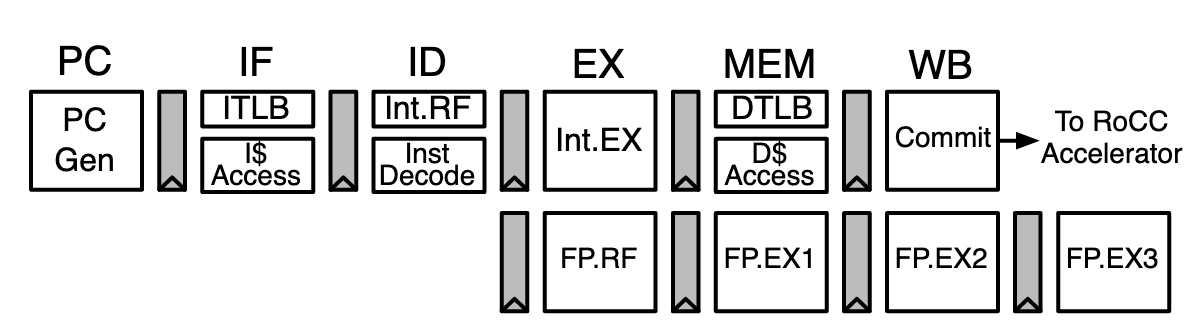
\includegraphics[scale=.4]{pngs/RocketPipeline.png}
    \caption{Rocket Chkp Pipeline\cite{Asanović:EECS-2016-17}}
    \label{fig:RocketCipFlow}
\end{figure}
The Rocket core is a RISC-V based processor. The basic core is a single fetch, single issue, in-order scalar processor, see figure \ref{fig:RocketCipFlow}. The basic core follows a subset of the RISC-V standard ??. The following is a list of the supported extensions: integer (I), multiply and divide (M), atomic (A), single-precision (F) and double-precision (D) floating point. This group of extensions is referred as (IMAFG) or (G) \cite{Asanović:EECS-2016-17}. In addition to S extension group, the Rocket core supports the E extension set. This set is used to communicate with the RoCC unit. % FIXME need to find ref for E extension

%The default RSIC-V Processor is called the Rocket Core. The Rocket Core is a single fetch, single issue, in-order scalar processor. The Rocket Core was designed to the RISC-V ISA standard. Figure \ref{fig:RocketCipFlow} show the basic flow of the Rocker Core. The basic version of the Rocket Core use the integer (I) extension. It can be configured to support additions extension: multiply and divide (M), atomics (A), single-precision (F) and double-precision (D) floating point\cite{Asanović:EECS-2016-17}. This set of extension are know as (IMAFD), or (G) extension\cite{Asanović:EECS-2016-17}. To support accelerators, the Rocket Core use the (E) extension. These set of instruction control the ROCC interface. The ROCC interface interfaces the Rocket Core and the ROCC Accelerator.
\subsection{Chisel}
The Rocket Chip Generator is written in Chisel. Chisel is a domain specific language (DSL) embedded in the Scala programming language. Chisel was developed and maintained by UCB. Chisel is used as a high level behavioral synthesis tools. Chisel allows the use of high level software constructs to drive hardware generation. It allows for complex port declarations and generate statements.   

%Chisel3 is an domain specific language (DSL) written Scala. Chisel is used to embed RTL in a high level language. It combines function program with hardware description. The Rocket Chip Generator is written in this DSL. One of the advantage to this DSL, is that port list can grow and shrink based off the configuration, and hardware generation can be controlled with complex function. This can be done with the use of defines in verilog, but it would not be salable. There would need to be a different define for each reparation of code. Interface can be used, but they can not be extended or reduced. Interface can be parameterized, but this function not wildly supported across all synthesis tools.  
\subsection{Configuring the Rocket Chip Generator}
All modules in the Rocket Chip Generator are passed a set of configuration. These configurations are passed down from top level module. At the top level, these configurations are appended together to create the generated design. Figure \ref{fig:configsnipit} shows how to add RoCC co-processor to the basic Rocket core. 


%The Rocket Chip Generator uses a set of configures to generator the Rocker Chip in verilog. Each module in the Rocket Chip Generator take a set of configuration. Depending on which set of configuration are set some module will be left out. For example, to have a accelerator added in a tile, extend the base configure and add the configuration for the accelerator. The main configuration file is located in the following directory: /src/main/scale/system/Config.scala. Figure \ref{fig:configsnipit} show an example of such a configuration.
\begin{figure}
    \centering
    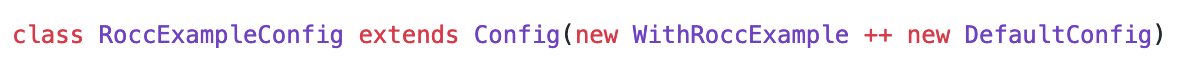
\includegraphics[scale=.4]{pngs/ConfigSnipit.png}
    \caption{ROCC Example Config}
    \label{fig:configsnipit}
\end{figure}
\end{document}